\chapter{Smap Transformation}

\label{ch:smap-transformation}

Aim of the smap transformation step is to merge a bounded number of fetches into a single fetch.
How many times the fetch would be executed is not known at compile time but only given at runtime by the length of the collection which is being mapped over.
Basis for the transformation itself is that a mapping operation over two composed functions is semantically identical to the composition one mapping operation with one function each, in the same order.

\begin{verbatim}
map (f . g) == map f . map g
\end{verbatim}

The basic transformation steps can be described as follows:

The function inside the map is separated into a computation before the fetch, the fetch, and a computation after the fetch.

\begin{verbatim}
map (after . fetch . before)
\end{verbatim}

We use the rule from above to separate the composed function into separate maps.

\begin{verbatim}
map after . map fetch . map before
\end{verbatim}

And finally we replace the \texttt{map fetch} by wrapping the list of requests we get from \texttt{before} in a request tree and fetch only that.

\begin{verbatim}
map after . mkList . fetch . mkTree . map before
\end{verbatim}

\section{Implementation detail}

The simplified explanation above is, albeit a nice and easy example, wrong.
Unfortunately, although it handles the case above correctly, it does not handle the general case correctly.
Not every computation is a simple pipeline, like displayed there, and thus could be broken into those three separate functions.
% A general case could be displayed using a tuple of the data for the fetch and the rest of the flowing data, like so
% map after . map (first fetch) . map before
% and then
% map after . uncurry zip . first (map fetch) . unzip . map before
We operate not in a normal programming language but on a dataflow graph which, in this case, is more powerful.
As a consequence we can separate out the fetch, wrap it, like described above, and batch it, even if there is other data flowing from \texttt{before} to \texttt{after} which does not pass through the \fetch{}.

On the dataflow IR we don't work with Clojure functions but with graph nodes, which could also be interpreted as operators.
The splitting is therefore not done with maps, but special nodes which start and end a mapping operation in Ohua.
The Ohua mapping operation is called \texttt{smap} and consists at IR level of several operators, the two interesting ones being \texttt{smap} (internally called \texttt{smap-fun}) and \texttt{collect}.
\texttt{smap} is the starting operator and provides the mapping functionality by continuously emitting items from a collection until the collection is empty.
\texttt{collect} is the opposite and only receives items until the collection is rebuilt.
Both also obtain information as to the size of the collection in order to function correctly.

The \texttt{smap} transformation as implemented in \yauhau{} simply inserts a collect operator before the fetch to rebuild the collection and a tree builder node to wrap it.
The collect operator is also fed the size of the original collection.
A new \texttt{smap} operator is inserted after the fetch to break the list into items again and continue the mapping.
A graphical example of this can be seen in Figure \ref{ch:smap-transformation}.

\begin{figure}[h]
	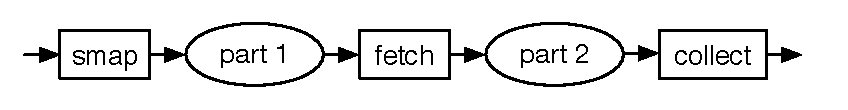
\includegraphics[width=.5\textwidth]{Figures/smap-rewrite-original}
	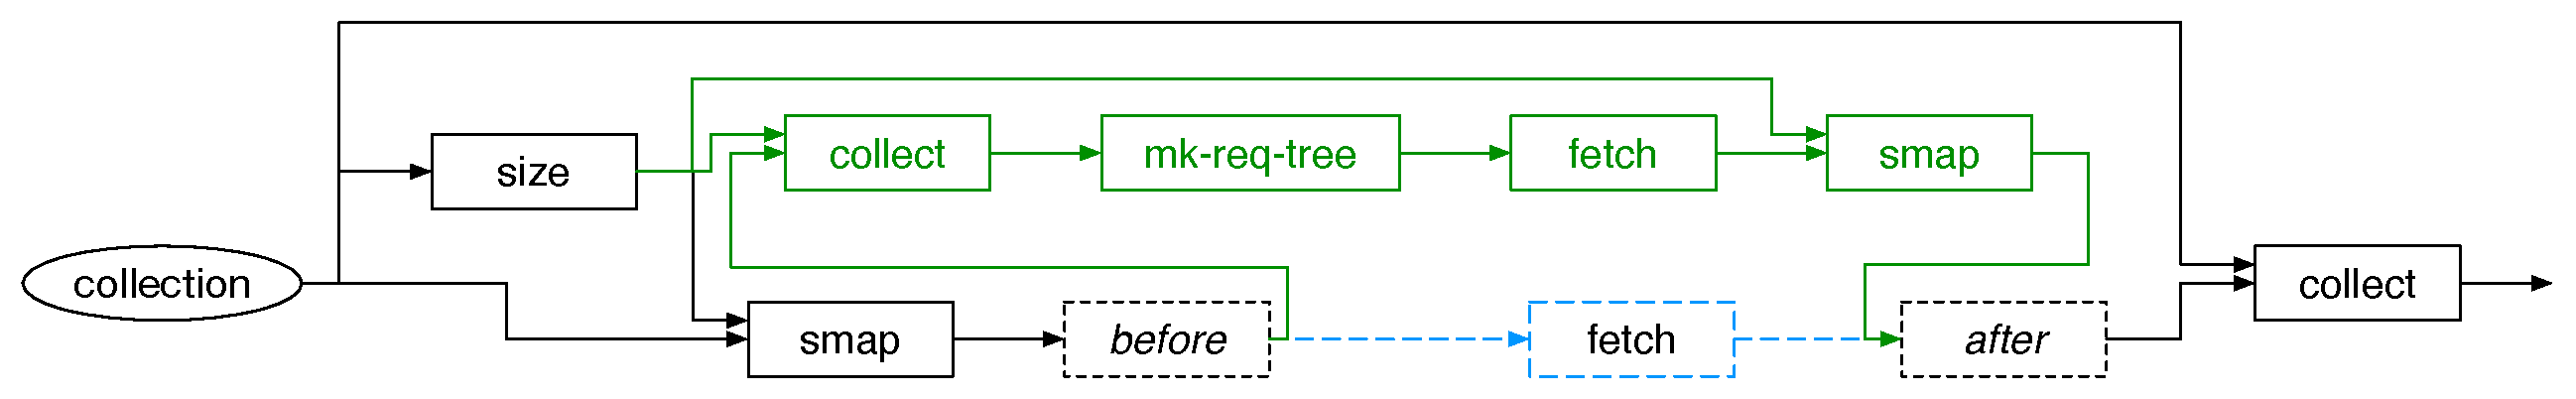
\includegraphics[width=.5\textwidth]{Figures/smap-rewrite}
	\label{figure:smap-transformation}
	\caption{Smap transformation}
\end{figure}

\section{Encoding}

The structure of the nested smap is saved in a tree structure.
We use an unlabeled rose tree.
It is important to use a tree structure because we would like to be able to support arbitrarily deep levels of nesting.
The Java programmer will recognise the Composite Pattern in the definition of our tree, which comprises of an abstract tree base class, Figure \ref{figure:tree-impl-base-class}.

\begin{figure}

\begin{minted}{Java}
public abstract class RequestTree {
    public abstract
    Stream<Request> getRequestsStream();

    public abstract
    Iterable<Object>
    buildResult(Map<Request, Object> responses);
}
\end{minted}
\caption{Abstract base class}
\label{figure:tree-impl-base-class}

\end{figure}

The basic tree offers methods to access all contained requests as a flat stream as well as a method for constructing a nested tree structure of results mirroring the structure of the request tree itself.
Our tree is composed of unlabeled branches which hold a sequence of subtrees as seen in Figure \ref{figure:tree-impl-branch}.
In this case the flat request stream simply comprises of the concatenation of all requests from the subtrees.
In this way we don't need any further knowledge of the structure of those subtrees to obtain the requests.
Although this structure is technically capable of handling a heterogeneous list of subtrees in practice, as a result of how these trees are created all subtrees have the same height and structure.

\begin{figure}

\begin{minted}{Java}
public final class RequestTreeBranch
             extends RequestTree {
    private final Iterable<RequestTree> subtrees;
    @Override
    public Stream<Request> getRequestsStream() {
        return StreamSupport
                  .stream(subtrees.spliterator(), false)
                  .flatMap(RequestTree::getRequestsStream);
    }

    @Override
    public
    Iterable<Object>
    buildResult(Map<Request, Object> responses) {
        return StreamSupport
                  .stream(subtrees.spliterator(), false)
                  .map(t -> t.buildResult(responses))
                  .collect(Collectors.toList());
    }
    /* omitted code */
}
\end{minted}
\caption{Concrete branch}
\label{figure:tree-impl-branch}

\end{figure}
\begin{figure}

\begin{minted}{Java}
public final class Request<P, R>
             extends RequestTree {
    @Override
    public Stream<Request> getRequestsStream() {
        return Collections
                 .singletonList((Request) this)
                 .stream();
    }

    @Override
    public
    Iterable<Object>
    buildResult(Map<Request, Object> responses) {
        return Collections.singletonList(responses.get(this));
    }
    /* omitted code */
}
\end{minted}

\caption{Request class}
\label{figure:tree-impl-request-class}
\end{figure}

Lastly our leaf nodes are simply requests, as the basic \texttt{Request} also extends the \texttt{RequestTree}, Figure \ref{figure:tree-impl-request-class}.

This rose tree encodes, in a data structure, the nested structure of the smap context.
The height of the tree equals the depth of smap nesting that was encoded.
